% !TEX encoding = UTF-8
% !TEX program = xelatex
\documentclass[12pt,a4paper]{article}
\usepackage[paperwidth=210mm, paperheight=297mm, left=0.75in, right=0.75in, bottom=1in, top=1in]{geometry}
\usepackage{polyglossia}
\setdefaultlanguage[babelshorthands]{italian}
\usepackage{fontspec}
\usepackage{graphicx}
\usepackage{blindtext}
\usepackage{wrapfig}

\frenchspacing
\makeindex

\begin{document}
\title{\vspace{-70pt}PIONEER 11}
\author{Michele Bianchi}
\date{}
\maketitle
\pagestyle{empty}
\thispagestyle{empty}

\section*{Storia}
\label{storia}
\begin{wrapfigure}{r}{0.35\textwidth}
  \vspace{-10pt}
  \begin{center}
    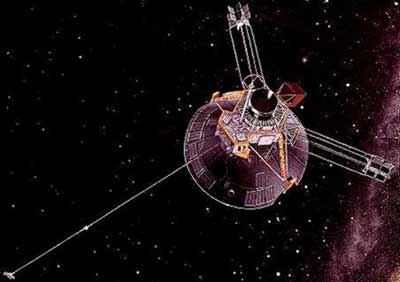
\includegraphics[width=0.30\textwidth]{satellite}
  \end{center}
  \vspace{-20pt}
\end{wrapfigure}
Dopo il Pioneer 10 il \textbf{Pioneer} 11 fu la seconda missione spaziale che raggiunse Giove e ed esplorò Saturno e i suoi anelli. Pioneer 11 utilizzò la massa di Giove per avere una spinta gravitazionale verso Saturno. Le comunicazioni con la sonda sono interrotte dal 30 Novembre 1995 a causa della grande distanza della sonda dalla Terra e a causa dell'energia sempre minore prodotta dal sistema di alimentazione.

È lunga 2,9 m ed ha un'antenna del diametro di 2,74 m che è stata utilizzata per comunicare con la Terra grazie all'ausilio del \emph{Deep Space Network}. Nella sonda sono presenti due generatori termoelettrici a radioisotopi che generavano 155 W di potenza elettrica al decollo e 140 al momento del flyby di Giove. La sonda necessitava di 100 watt per alimentare tutti i sistemi. Grazie a tre sensori denominati ``tracciatori di stelle'' (star-tracker), dei quali uno aveva come riferimento Canopus e due il Sole, era possibile determinare l'orientamento della sonda. Tale orientamento poteva essere modificato tramite l'attivazione di sei propulsori, di cui due controllavano la velocità di rotazione, due la spinta in avanti e due l'altitudine.

\section*{Osservazioni}
\label{osservazioni}

I suoi strumenti scientifici studiavano i campi magnetici planetari e interplanetari, le proprietà del vento solare, i raggi cosmici, la distribuzione, composizione, massa e velocità della polvere cosmica, le atmosfere e le superfici dei pianeti e dei satelliti.

\section*{Curiosità}
\label{curiosit}

Come la sua nave-sorella Pioneer 10, anche Pioneer 11 porta una placca dorata con dei messaggi indirizzati a una \textbf{intelligenza aliena}. Sono riportate informazioni sulla costruzione della sonda stessa, e disegni schematizzati di un uomo e una donna, e la posizione della Terra rispetto al Sole e del Sole nella Galassia.

\end{document}